\documentclass[12pt]{beamer}

\usetheme{Oxygen}
\usepackage{thumbpdf}
\usepackage{wasysym}
% \usepackage{ucs}
\usepackage[utf8]{inputenc}
\usepackage{pgf,pgfarrows,pgfnodes,pgfautomata,pgfheaps,pgfshade}
\usepackage{verbatim}
\usepackage{multicol}


\pdfinfo
{
  /Title       (Desarrollo Web)
  /Creator     (TeX)
  /Author      (Sebastián Salazar Molina)
}


\title{Desarrollo Web}
\subtitle{Mobile First}
\author{Sebastián Salazar Molina.}
\institute[INF - UTEM] { Unidad de Informática - Universidad Tecnológica Metropolitana }
\date{27 de Abril de 2014}

\begin{document}

\frame{\titlepage}

\section*{}
\begin{frame}
  \frametitle{Contenidos}
  \begin{multicols}{2}
    \tableofcontents[section=1,hidesubsections]
  \end{multicols}
\end{frame}

\AtBeginSection[]
{
  \frame<handout:0>
  {
    \frametitle{Contenidos}
    \begin{multicols}{2}
    \tableofcontents[currentsection,hideallsubsections]
    \end{multicols}
  }
}

\AtBeginSubsection[]
{
  \frame<handout:0>
  {
    \frametitle{Contenidos}
%     \begin{multicols}{2}
    \tableofcontents[sectionstyle=show/hide,subsectionstyle=show/shaded/hide]
%     \end{multicols}
  }
}

\newcommand<>{\highlighton}[1]{%
  \alt#2{\structure{#1}}{{#1}}
}

\newcommand{\icon}[1]{\pgfimage[height=1em]{#1}}



%%%%%%%%%%%%%%%%%%%%%%%%%%%%%%%%%%%%%%%%%
%%%%%%%%%% Content starts here %%%%%%%%%%
%%%%%%%%%%%%%%%%%%%%%%%%%%%%%%%%%%%%%%%%%



% Introducción
\section{Introducción}
\subsection{Introducción}

\begin{frame}
\frametitle{Acerca de mí.}
\begin{itemize}
 \item<2-> Sebastián Alexis Salazar Molina (@sebastian\_sm) .
 \item<3-> Ingeniero Civil en Computación (UTEM).
 \item<4-> Consultor TI en \href{http://www.experti.cl}{ExperTI} (C/C++ , PHP, Java)
 \item<5-> \href{http://sebastian.cl}{http://sebastian.cl}
\end{itemize}
\end{frame}


\section{Consejos}

\begin{frame}
 \frametitle{Adaptabilidad}
 La web es cada vez más compleja, y cada vez hay que cubrir una mayor cantidad de dispositivos resoluciones y características. 
 \newline
 Ante este desafío, el ``responsive web design'' nos entrega una herramienta flexible que nos permitirá adaptarnos ante las distintas circunstancias.
\end{frame}


\begin{frame}
 \frametitle{Contenido}
 El Usuario móvil, necesita el contenido ``{\bf esencial}'', bien distribuido, ordenado y fácil de navegar.
\end{frame}

\begin{frame}
 \frametitle{HTML5}
 Muchos navegadores móviles, sacan el máximo de partido de html5, por esta razón, tener una estructura ordenado, tener una semántica pulida y utilizar correctamente las etiquetas (usar los input html5), simplificará la tarea de adopción.
\end{frame}

\begin{frame}
 \frametitle{Viewport}
 Una buena idea, es ajustar el ancho de la página, al ancho del dispositivo, esto lo podemos lograr con:
 \begin{center}
    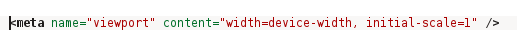
\includegraphics[scale=0.75]{img/viewport.png}
 \end{center}
\end{frame}


\begin{frame}
 \frametitle{Fragmentos}
 Para mejor la experiencia móvil, es importante disponer de contenido fragmentado, que sea ligero de incluir y que cargue rápido.
\end{frame}


\begin{frame}
 \frametitle{Aprovechar HTML5}
 Un truco interesante para crear contenido móvil, es disminuir la cantidad de imágenes necesarias para que se visualice nuestro sitio. Para esto podemos usar caracteres especiales de HTML, lo típico, de un comentario con estrellas se puede usar con \&\#9733; y \&\#9734;
 \newline
 http://dev.w3.org/html5/html-author/charref
\end{frame}


\begin{frame}
 \frametitle{Teléfono}
 Algo que se valora mucho, es la opción de brindar la posibilidad de hacer una llamada desde nuestro teléfono, demosle la opción a nuestros usuarios:
 \begin{center}
    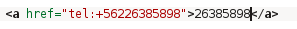
\includegraphics[scale=1]{img/tel.png}
 \end{center}
\end{frame}


\begin{frame}
 \frametitle{Estilos}
 Es importante separar los estilos, en función de las resoluciones soportadas.
 \begin{center}
    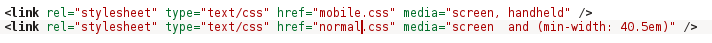
\includegraphics[scale=0.5]{img/estilo.png}
 \end{center}
\end{frame}



\frame{
  \vspace{2cm}
  {\huge ¿ Preguntas ?}

  \vspace{3cm}
  \begin{flushright}
    Sebastián Salazar Molina

    \structure{\footnotesize{@sebastian\_sm}}
  \end{flushright}
}

\end{document}
